\chapter{Trout Recipes}

In this chapter we intend to publish Trout Recipes for dishes that have been 
attempted at Mbona. Please email your trout recipes to the editor at:

\href{mailto:hugh.murrell@gmail.com}{hugh.murrell@gmail.com}

Your recipe can be in plain text with an {\bf ingrediants} section
and an {\bf instructions} section. Please attach a photo of the resulting
dish just before eating commences. See our braai trout recipe for an example.

\clearpage


\section{Robertson's Braai Trout  (by Hugh Murrell)}

\subsection*{ingredients}

\begin{itemize}
\item 2 Whole Trout, gilled and gutted.
\item Robertsons Spice for Fish
\item 2 lemons
\item 1 Fennel Bulb
\item 1 lemon
\item For the Yogurt Dressing:
\begin{itemize}
\item 250ml Greek Yogurt, double cream
\item 45ml mayonnaise
\item 1 lemon, juiced
\item 10ml Wholegrain Mustard
\item Robertsons Coarsely Ground Black Pepper
\end{itemize}
\end{itemize}

\subsection*{instructions}

\begin{itemize}
\item Get your fire ready to braai the fish over medium hot coals.
\item Oil the inside of your grid to ensure that the fish doesn't stick to the grid.
\item Rinse the trout well under cold water, then pat dry with a tea towel.
\item Season the fish, inside and outside, with Robertsons Spice for Fish. 
\item Use lemon and sliced fennel slices to stuff into the cuts and cavity, 
then drizzle the stuffed parts with lemon juice. 
\item Place the fish inside a large hinged grid (without any foil) 
using a few lemon slices to protect the fish, see figure \ref{fig:braaiTroutPrepared}


 
\item braai over medium hot coals on both sides for about 30 minutes in total, see figure \ref{fig:braaiTroutPrepared}.


\item For the dressing, mix all the ingredients together.
\item Transfer the fish to a large serving platter and serve with a bowl of yogurt dressing, see figure \ref{fig:braaiTroutServed}

\end{itemize}

\subsection*{results}
  
\begin{figure}[H]
\centering
  \includegraphics[scale=0.25]{recipes/braaiTroutPrepared.jpg} \hspace{1cm}  \includegraphics[scale=0.25]{recipes/braaiTroutCooking.jpg}
   \caption{Robertson's Braai Trout, prepared (left image) and on the coals (right image)}
  \label{fig:braaiTroutPrepared}
\end{figure}  


\begin{figure}[H]
\centering
  \includegraphics[scale=0.2]{recipes/braaiTroutServed.jpg}
   \caption{Robertson's Braai Trout, served and ready to be eaten.}
  \label{fig:braaiTroutServed}
\end{figure}

\section{Smoking Bag Trout (by Andrew Johnson)}

\subsection*{ingredients}
\begin{itemize}
\item 1 Large Trout, gilled and gutted.
\item 1 SAVU Smoker Bag (imported from Finland)
\item coarse salt
\item olive oil
\item Robertsons Spice for Fish
\item many knobbly limes 
\end{itemize}

\subsection*{instructions}
\begin{itemize}
\item catch one large trout.
\item gill and gut trout without removing head or tail
\item salt trout inside and out and leave in fridge overnight
\item wash and dry trout
\item coat outside with tiny portion of olive oil
\item spice inside and out with Robertsons Spice for Fish
\item fill cavity with lime zest and red peppers
\item place trout inside smoker bag and seal bag tightly
\item pre-heat gas oven to over 250 C
\item place bag in hot oven at lowest position with "this side down" down
\item cook at 250 for first 15 minutes and then at 190 for 30 minutes (do NOT turn the bag).
\item take bag from the oven using oven mitts and let trout rest for 5 min before serving
\item cut open top of bag with sissors and turn foil to side
\item remove trout skin with sharp knife and slide trout flesh into warm serving dish
\end{itemize}

\subsection*{results}
  
\begin{figure}[H]
\centering
  \includegraphics[scale=0.17]{recipes/HotSmoked1.jpg} \hspace{1cm}    \includegraphics[scale=0.05]{recipes/HotSmoked2.jpg}
   \caption{Large Trout (left image) and SAVU smoking bag (right image)}
  \label{fig:HotSmokedTrout}
\end{figure}  


\begin{figure}[H]
\centering
  \includegraphics[scale=0.15]{recipes/HotSmoked3.jpg} \hspace{1cm}  \includegraphics[scale=0.15]{recipes/HotSmoked4.jpg}
   \caption{Opened Bag (left image) and serving dish (right image)}
  \label{fig:HotSmokedTroutServed}
\end{figure}


\newpage
\section{Citrus Braai Trout (by Soula Contogiannis)}

\subsection*{ingredients for one trout}

\begin{itemize}
\item 3 layers of heavy duty foil
\item 1 trout
\item red or white grapes or rasins
\item 2 by orange or lemon slices plus juice 
\item fresh mint
\item 2 cloves of garlic
\item onion slices
\item fresh dill or three chillies
\item olive oil and butter
\item salt and pepper to taste
\end{itemize}

\subsection*{instructions}

\begin{itemize}
\item rub trout with olive oil, salt and pepper. 
\item fill cavity with citrus slices, onion rings, mint and dill or chillie.
\item sprinkle grapes or rasins on and around trout. 
\item place citrus slices and cubes of butter on top of trout.
\item pour citrus juice over trout
\item seal the trout in the foil making sure that there are no openings. 
\item place on a braai with hot coals. 
\item cook for approximately 1 hour or until a skewer used to poke through the foil goes in easily with no resistance.
\end{itemize}

\subsection*{results}
  
\begin{figure}[H]
\centering
  \includegraphics[scale=0.15]{recipes/soula_6.jpg} \hspace{0.2cm}  \includegraphics[scale=0.15]{recipes/soula_7.jpg} \\ \vspace{0.2cm}
  \includegraphics[scale=0.15]{recipes/soula_3.jpg} \hspace{0.2cm}
    \includegraphics[scale=0.15]{recipes/soula_4.jpg} \\ \vspace{0.2cm}
    \includegraphics[scale=0.15]{recipes/soula_2.jpg} \hspace{0.2cm}   \includegraphics[scale=0.15]{recipes/soula_5.jpg} 
   \caption{Soula's Citrus Braai Trout, gutted and prepared for Braai}
  \label{fig:SoulaBraaiTrout}
\end{figure}  

\newpage
\section{Whole Baked Trout with Herb Salsa \\ (by Natasha Russo)} 

thanks to,  \url{http://eatdrinkpaleo.com.au/whole-baked-trout-recipe/}

\subsection*{ingredients for two trout}

\begin{itemize}
\item 2 Whole Trout, gilled, gutted and heads and tails removed.
\item For the salsa
	\begin{itemize}
		\item 1 medium red onion, peeled and roughly diced
		\item A handful of fresh basil leaves
		\item A handful of fresh parsley
		\item A few mint leaves
		\item 1 garlic clove, peeled
		\item Zest of 1 lemon
		\item Juice of half lemon 
		\item half cup olive oil
		\item 2 teaspoon sea salt
		\item half teaspoon black pepper
	\end{itemize}
\end{itemize}

\subsection*{instructions}

\begin{itemize}
	\item Preheat the oven to 200 centegrade
	\item Combine the salsa ingredients in a food processor or a blender and process into a salsa like consistency.
	\item Remove Heads and Tails and place the whole fish in a large roasting tray. 
	\item Cover the fish with the herb marinade on both sides and a little inside the fish cavity. 
	\item Bake in the oven for 20-25 minutes, on the middle shelf. 
	\item Remove and transfer to a platter or serve right in the roasting tray.
	\item Best with Spinach, Cranberry and Roast Almond Salad
\end{itemize}

\subsection*{results}
  
\begin{figure}[H]
\centering
  \includegraphics[scale=0.12]{recipes/NatashaPrepared.jpg} \hspace{1cm}  \includegraphics[scale=0.12]{recipes/NatashaPrecooked.jpg}
   \caption{Whole Trout, gutted (left image) and prepared (right image)}
  \label{fig:NatashaPrepared}
\end{figure}  

\begin{figure}[H]
\centering
  \includegraphics[scale=0.2]{recipes/NatashaServed.jpg}
   \caption{Natasha's Whole Baked Trout, served and ready to be eaten.}
  \label{fig:NatashaServed}
\end{figure}

\section{Mbona Cold Smoked Trout \\ (by Dave Forsyth and Guy Reen)} 

\subsection*{Ingredients}

\begin{itemize}
\item as many gutted and cleaned trout as fill fit in your smoker.
\item healthy supply of coarse salt
\item very sharp filleting knife
\item pin bone tweezers
\item indoor hanging space
\item cold smoking kiln
\item wood chips
\item vacuum packer
\end{itemize}

\subsection*{instructions}

\begin{itemize}
	\item Fillet the trout, fig \ref{fig:SmokingProceedure}A
	\item Dry and salt fillets librally.
	\item after 2 hours, wash salt off fillets and dry.
	\item hang fillets indoors overnight with fan running, fig \ref{fig:SmokingProceedure}B
	\item light wood chips and allow smoke to enter chamber from a distance, fig \ref{fig:SmokingProceedure}C
	\item place fillets in smoking chamber, fig \ref{fig:SmokingProceedure}D
	\item smoke for 2.5 hours (as long as wood chips last)
	\item remove pin bones, fig \ref{fig:SmokingProceedure}E
	\item vacuum pack fillets, fig \ref{fig:SmokingProceedure}F
\end{itemize}

\subsection*{results}
  
\begin{figure}[H]
\centering
\includegraphics[height=120pt]{recipes/smoking/RainbowFillets.jpg} \includegraphics[height=120pt]{recipes/smoking/SaltedFillets.jpg} \\
\includegraphics[height=140pt]{recipes/smoking/SmokingApparatus.jpg} \includegraphics[height=140pt]{recipes/smoking/FilletChamber.jpg} 
\includegraphics[height=140pt]{recipes/smoking/RemovingPinBones.jpg} \\
\includegraphics[height=180pt]{recipes/smoking/VacumePacked.jpg} 
   \caption{Smoking proceedure: A: Rainbow fillets, B: salted trout fillets hanging, C: apparatus with burning wood chips some distance from smoking chamber, D: fillets in smoking chamber, E: removing the pin bones, F: vacuum packed and ready for sale}
  \label{fig:SmokingProceedure}
\end{figure}  

\section{Smoked Trout with Cucumber Mousse \\ (by Dave Forsyth)}

\subsection*{ingredients}

\begin{itemize}
\item 1 Mbona smoked trout fillet
\item 1 packet of savoury biscuits
\item and for the mousse
\begin{itemize}
\item 1 greengage jelly (or 1 envelope gelatin)
\item 1 peeled and grated cucumber 
\item mayonaise and full cream
\item white vinegar, chopped mint, grated onion, horse-radish source
\end{itemize}
\end{itemize}

\subsection*{instructions}

\begin{itemize}
\item slice byte size medallions from Trout fillet.
\item for the mousse
\begin{itemize}
\item add jelly to 284 ml boiling water
\item add 2T white vinigar and allow to start setting
\item add whole grated cucumber 
\item add 1T chopped mint, 1T grated onion and 1t horse-radish source.
\item add 1c mayonaise/cream mixture
\item place in fish mould and refrigerate
\end{itemize}
\item arrange trout medallions and biscuits on one plate and upend cucumber mousse on another plate and serve as shown in figure \ref{fig:daveStarter}
\end{itemize}

\subsection*{results}
  
\begin{figure}[H]
\centering
  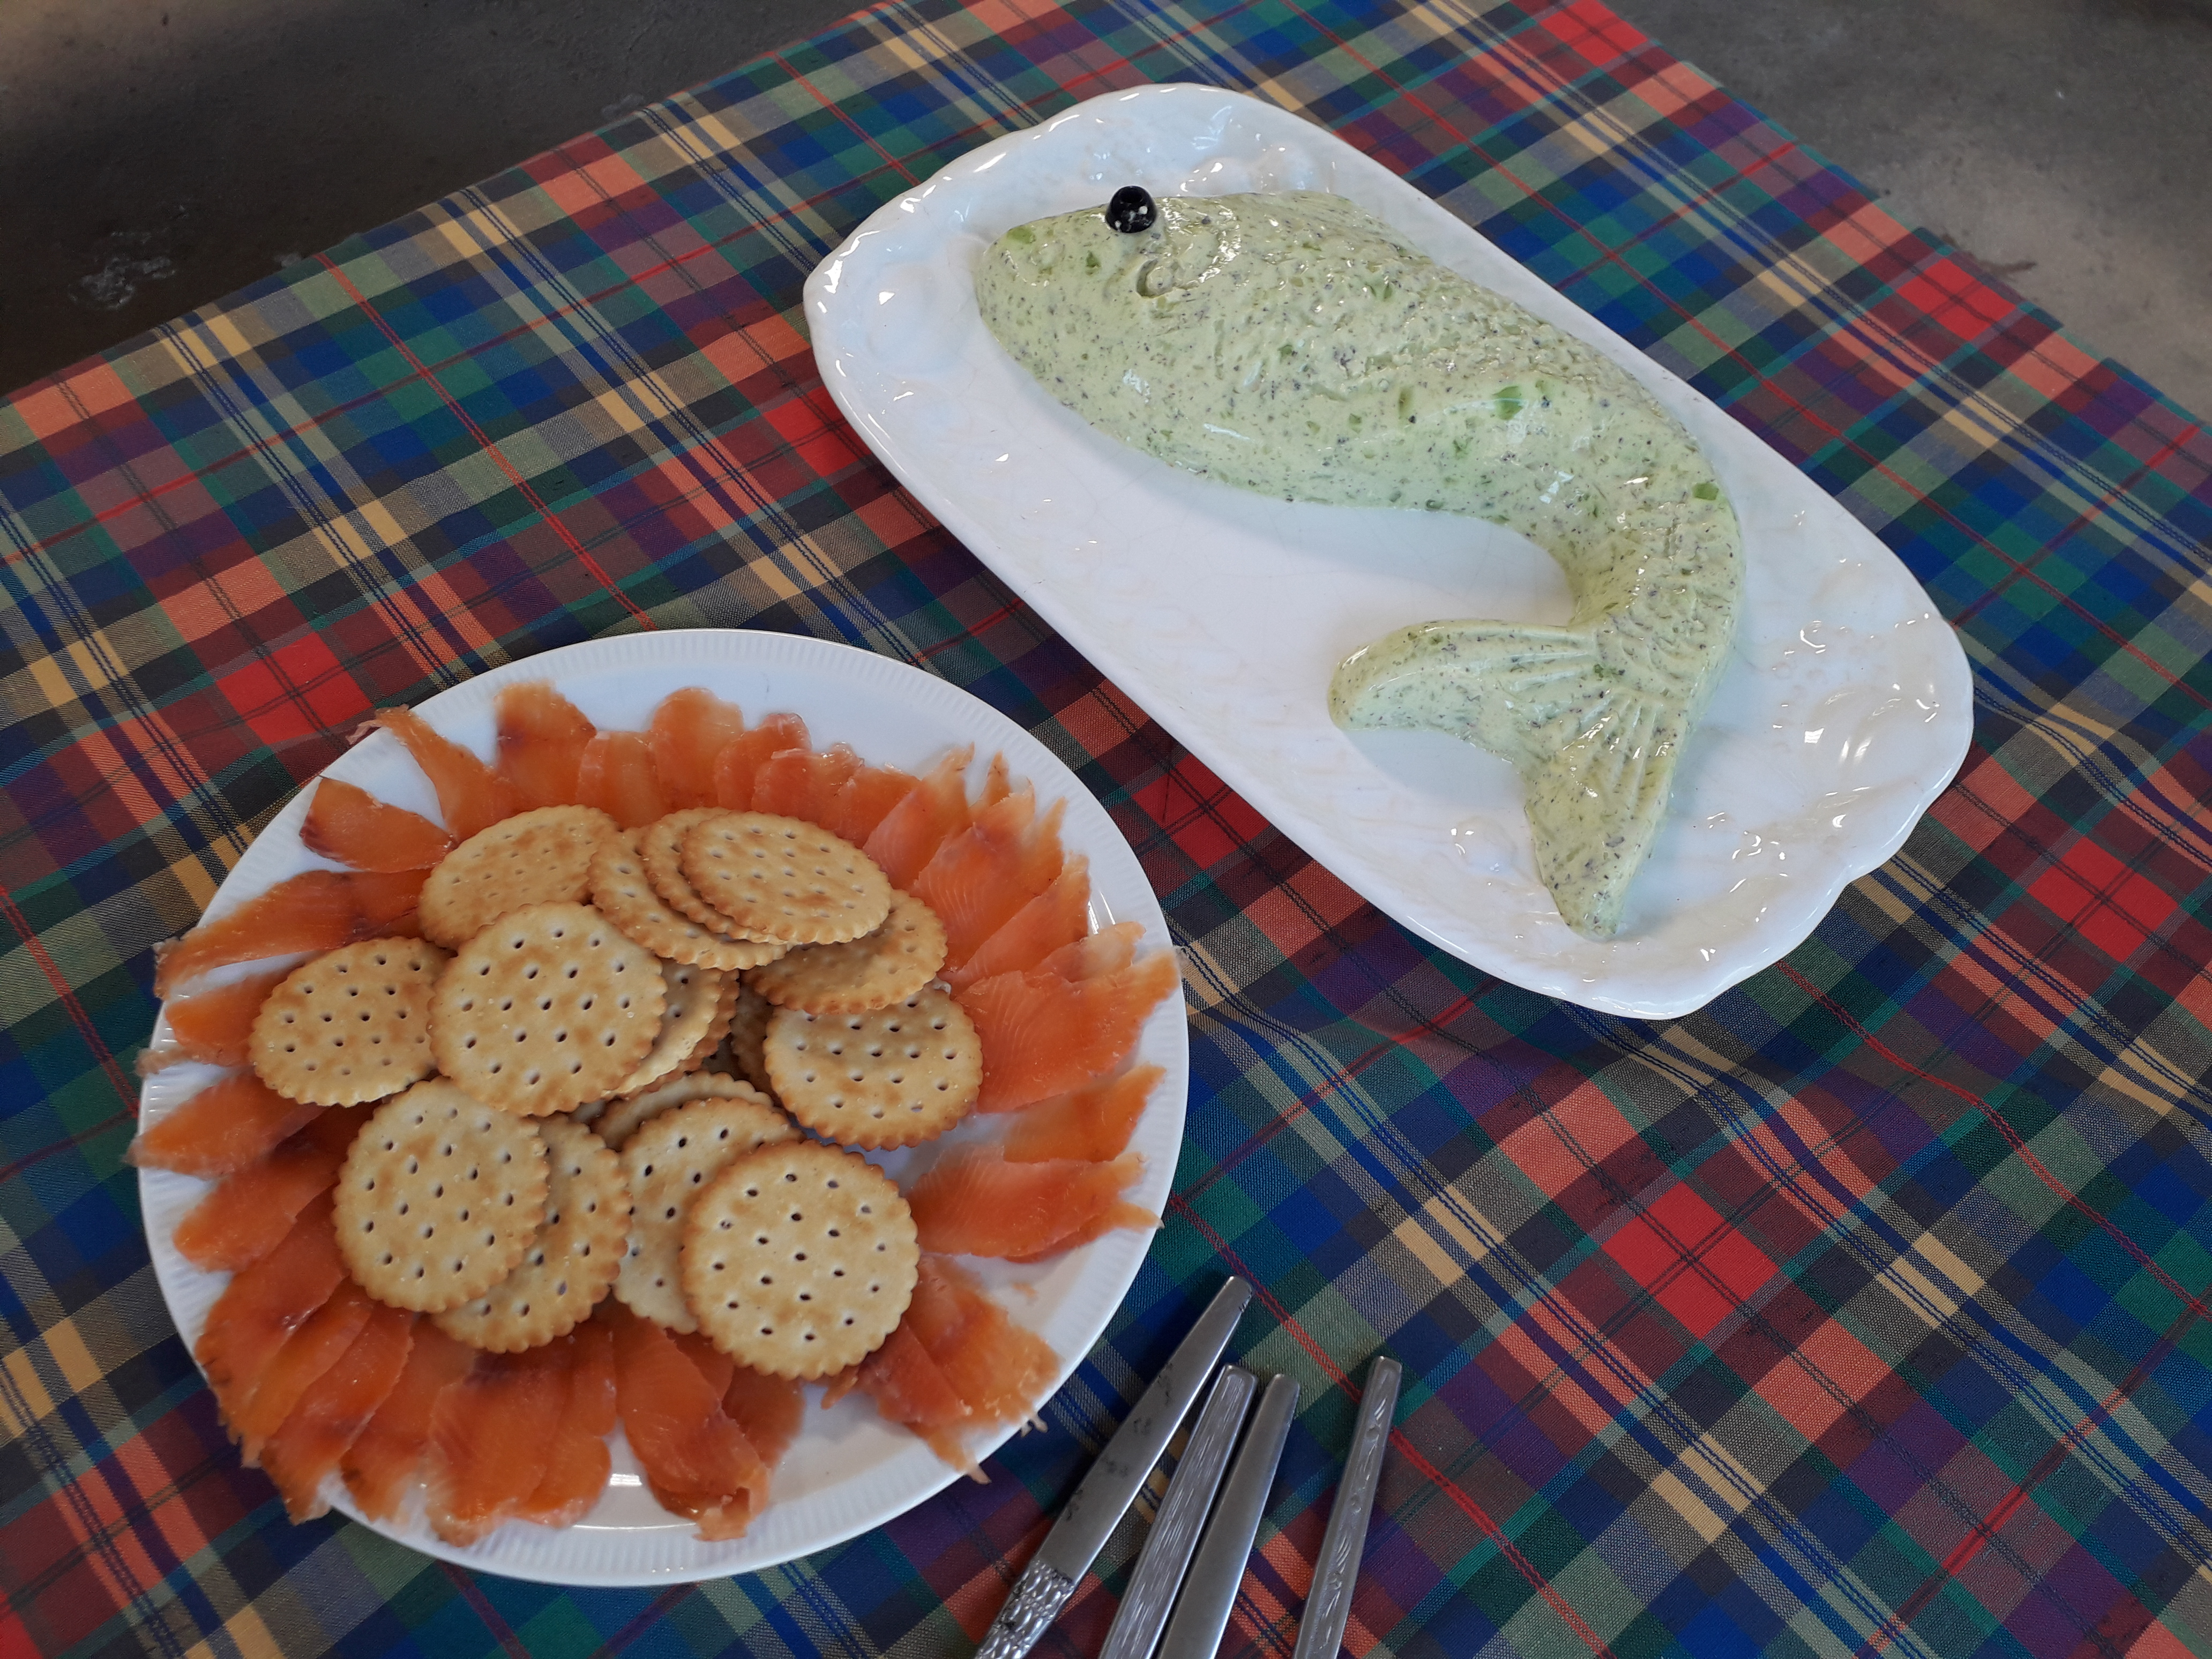
\includegraphics[scale=0.1]{recipes/DaveSmokedTroutWithCucumberMousse.jpg} 
     \caption{Dave's Smoked Trout with Cucumber Mousse starter}
  \label{fig:daveStarter}
\end{figure}  

